% XCircuit output "cto_1.tex" for LaTeX input from cto_1.eps
\def\putbox#1#2#3#4{\makebox[0in][l]{\makebox[#1][l]{}\raisebox{\baselineskip}[0in][0in]{\raisebox{#2}[0in][0in]{\scalebox{#3}{#4}}}}}
\def\rightbox#1{\makebox[0in][r]{#1}}
\def\centbox#1{\makebox[0in]{#1}}
\def\topbox#1{\raisebox{-0.60\baselineskip}[0in][0in]{#1}}
\def\midbox#1{\raisebox{-0.20\baselineskip}[0in][0in]{#1}}
   \scalebox{1}{
   \normalsize
   \parbox{10.3125in}{
   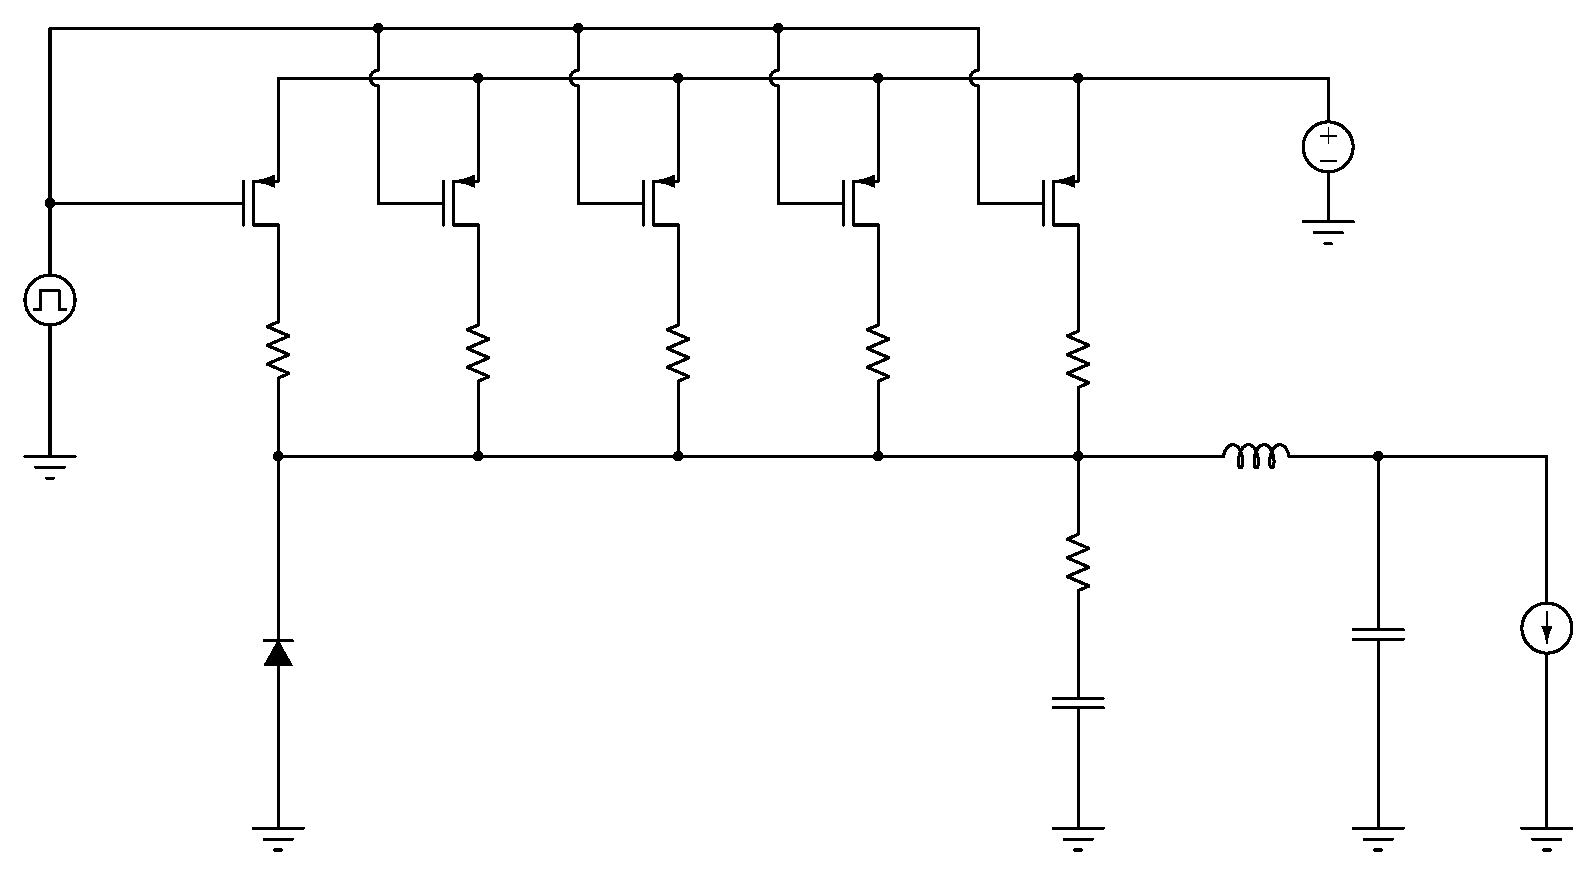
\includegraphics[scale=1]{cto_1}\\
   % translate x=836 y=860 scale 0.38
   \putbox{1.72in}{4.31in}{1.20}{M1}%
   \putbox{3.06in}{4.31in}{1.20}{M2}%
   \putbox{4.39in}{4.31in}{1.20}{M3}%
   \putbox{5.72in}{4.31in}{1.20}{M4}%
   \putbox{7.06in}{4.31in}{1.20}{M5}%
   \putbox{1.41in}{3.31in}{1.20}{R1}%
   \putbox{2.66in}{3.31in}{1.20}{R2}%
   \putbox{3.97in}{3.31in}{1.20}{R3}%
   \putbox{5.33in}{3.31in}{1.20}{R4}%
   \putbox{6.68in}{3.24in}{1.20}{R5}%
   \putbox{1.85in}{3.31in}{1.20}{0,5}%
   \putbox{3.18in}{3.31in}{1.20}{0,5}%
   \putbox{4.51in}{3.29in}{1.20}{0,5}%
   \putbox{5.87in}{3.31in}{1.20}{0,5}%
   \putbox{7.18in}{3.29in}{1.20}{0,5}%
   \putbox{1.93in}{1.29in}{1.20}{D1}%
   \putbox{8.22in}{4.87in}{1.20}{V1}%
   \putbox{8.20in}{4.54in}{1.20}{12V}%
   \putbox{0.49in}{3.79in}{1.20}{12V}%
   \putbox{0.47in}{3.54in}{1.20}{20kHz}%
   \putbox{8.08in}{2.95in}{1.20}{L1}%
   \putbox{7.99in}{2.37in}{1.20}{$10 \mu$}%
   \putbox{8.54in}{1.45in}{1.20}{C1}%
   \putbox{8.45in}{1.20in}{1.20}{$1m$}%
   \putbox{6.62in}{1.95in}{1.20}{R6}%
   \putbox{7.26in}{1.95in}{1.20}{100}%
   \putbox{6.51in}{0.99in}{1.20}{C3}%
   \putbox{7.35in}{0.97in}{1.20}{$5n$}%
   \putbox{9.70in}{1.47in}{1.20}{2A}%
   } % close 'parbox'
   } % close 'scalebox'
   \vspace{-\baselineskip} % this is not necessary, but looks better
